\documentclass{beamer}
\usepackage{beamerthemesplit}
\usepackage{graphicx}
\usepackage{listings}
\usepackage{fancyvrb}
\usepackage{color}

\lstset{
    fancyvrb=true,
    basicstyle=\normalfont
}

\begin{document}

\begin{frame}
    \frametitle{dnode: freestyle rpc}
    \begin{center}
        
\includegraphics[scale=0.3]{images/freestyle_turtle.png}
    \end{center}
\end{frame}

\begin{frame}
    \begin{center}
        \frametitle{asynchronous sky cake}
        \huge

        dnode makes stringing together processes easy as cake
        \newline

        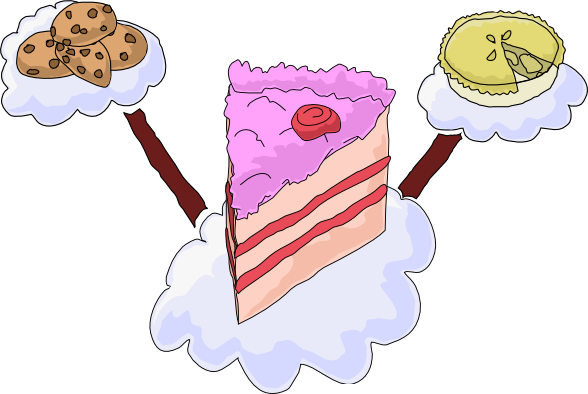
\includegraphics[scale=0.5]{images/sky_cake.png}
    \end{center}
\end{frame}

\begin{frame}
    \frametitle{zing server}

    \huge
    just hack up a server
    \newline

    \normalsize
    \fbox{\lstinputlisting{code/zing/server.js}}
\end{frame}

\begin{frame}
    \frametitle{zing client}

    \huge
    then call the server's .zing() in your client!
    \newline

    \normalsize
    \fbox{
        \lstinputlisting{code/zing/client.js}
    }
\end{frame}

\begin{frame}
    \frametitle{none of this noise}
    
    \begin{columns}[c]
    \column{.2\textwidth}
        
\includegraphics[scale=0.4]{images/no.png}
    \column{.8\textwidth}
        \huge
        \begin{itemize}
            \item No schemas
            \item No XML
            \item No custom dispatching
        \end{itemize}
        \pause
        Just call functions!
    \end{columns}
\end{frame}

\begin{frame}
    \frametitle{client and server side by side}
    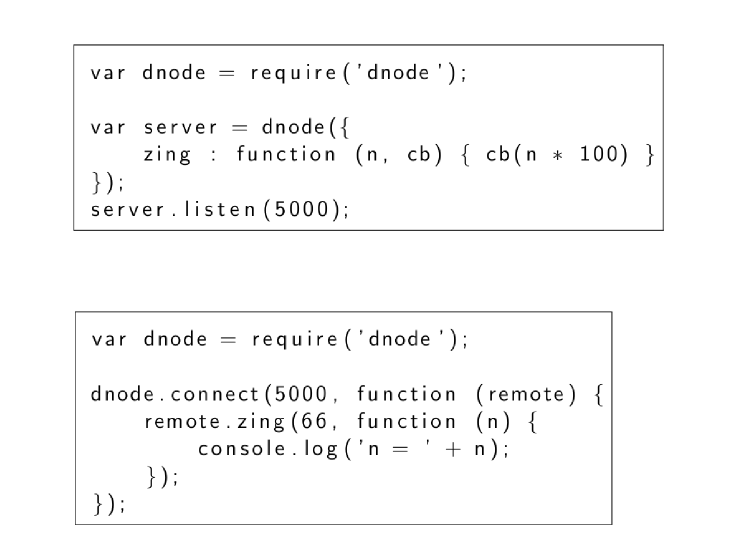
\includegraphics[scale=0.6]{images/zing_flow_0.png}
\end{frame}

\begin{frame}
    \frametitle{pass along n...}
    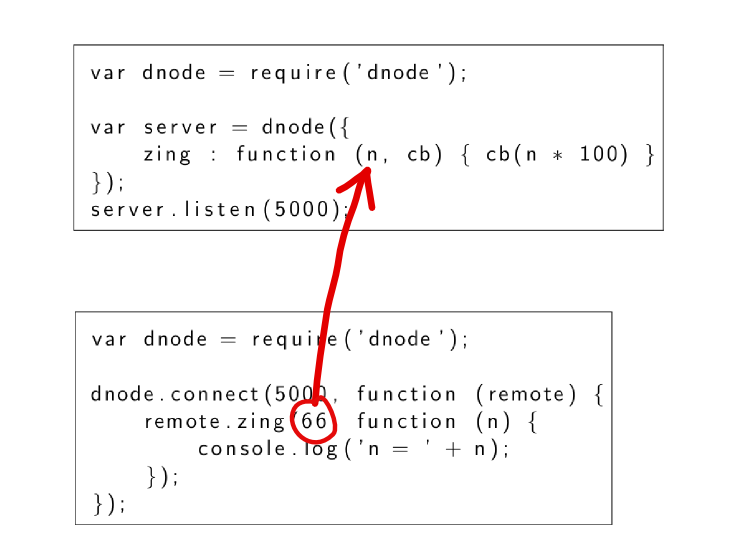
\includegraphics[scale=0.6]{images/zing_flow_1.png}
\end{frame}

\begin{frame}
    \frametitle{pass along the cb...}
    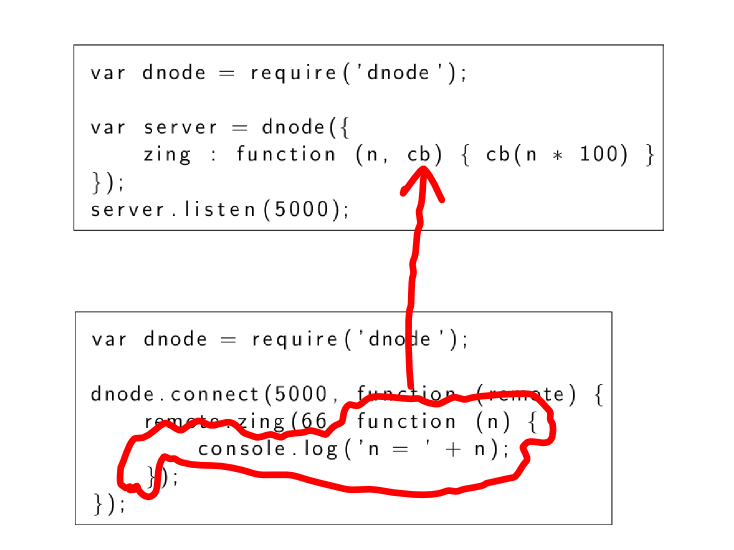
\includegraphics[scale=0.6]{images/zing_flow_2.png}
\end{frame}

\begin{frame}
    \frametitle{then just call the cb...}
    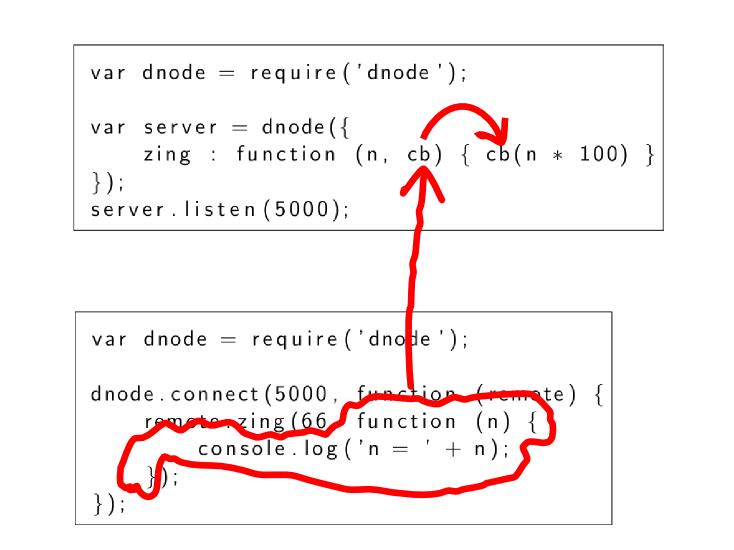
\includegraphics[scale=0.6]{images/zing_flow_3.png}
\end{frame}

\begin{frame}
    \frametitle{with the parameters you passed in...}
    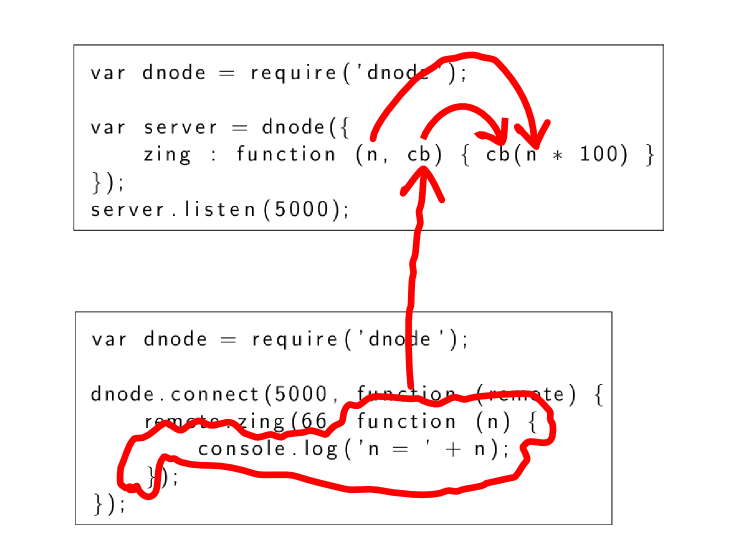
\includegraphics[scale=0.6]{images/zing_flow_4.png}
\end{frame}

\begin{frame}
    \frametitle{and your callback gets the result...}
    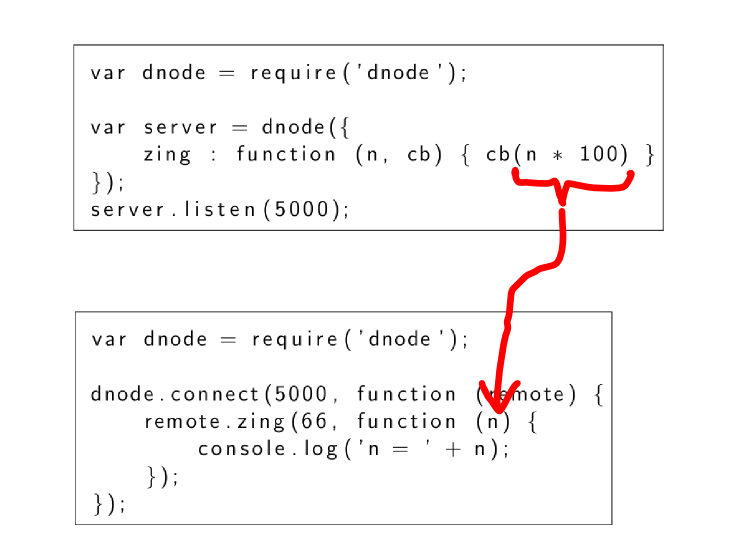
\includegraphics[scale=0.6]{images/zing_flow_5.png}
\end{frame}

\begin{frame}
    \frametitle{which you can use for whatevs}
    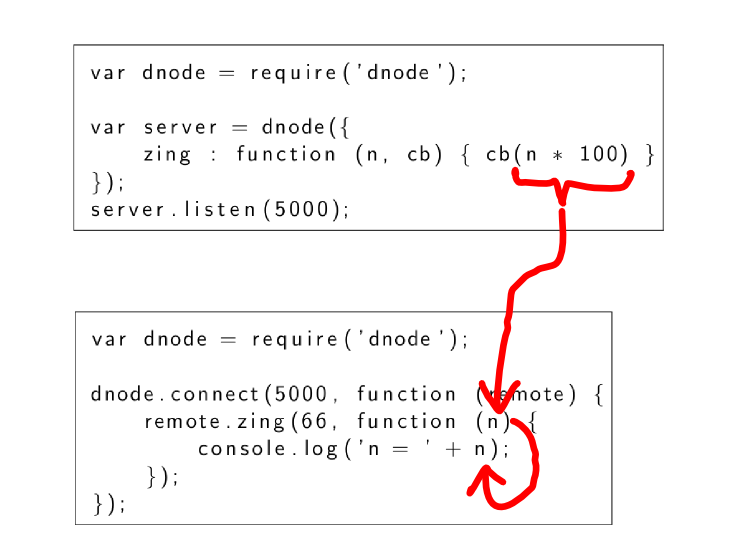
\includegraphics[scale=0.6]{images/zing_flow_6.png}
\end{frame}

\begin{frame}
    \frametitle{that's all it takes!}
    \begin{center}
        \fbox{\lstinputlisting{code/zing/output}}
    \end{center}
\end{frame}

\begin{frame}
    \frametitle{fuck yeah, callbacks!}
    \begin{center}
        
\includegraphics[scale=0.4]{images/fuck_yeah.png}
        \newline
        \pause
        \huge
        Now let's do that in the browser.
    \end{center}
\end{frame}

\begin{frame}
    \frametitle{zing web server}
    
    \huge
    web server
    \newline
    
    \normalsize
    \fbox{\lstinputlisting{code/browser/server.js}}
\end{frame}

\begin{frame}
    \frametitle{zing tcp \& web server why not}
    
    \huge
    network and web server
    \newline
    
    \normalsize
    \fbox{\lstinputlisting{code/browser/both.js}}
\end{frame}

\begin{frame}
    \frametitle{zing web client}
    \huge
    just hack up an index.html:
    \newline
    
    \scriptsize
    \fbox{\lstinputlisting{code/browser/index.html}}
\end{frame}

\begin{frame}
    \frametitle{zing web output}
    \large
    by the power vested in me by socket.io...
    \newline
    
    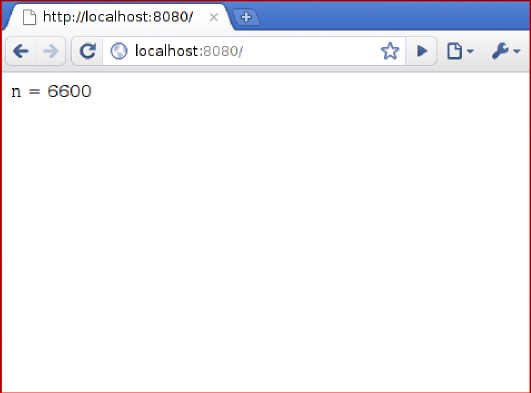
\includegraphics[scale=0.6]{images/browser.png}
\end{frame}

\begin{frame}
    \frametitle{browserify!}
    
    \huge
    dnode works great with browserify out of the box
    for client-side require()
    \newline
    
    \begin{center}
        
\includegraphics[scale=0.35]{images/browserify.png}
    \end{center}
\end{frame}

\begin{frame}
    \frametitle{browserify server}
    
    \begin{center}
        \scriptsize
        \fbox{\lstinputlisting{code/browserify/server.js}}
    \end{center}
\end{frame}

\begin{frame}
    \frametitle{browserify index.html}
    
    \begin{center}
        \scriptsize
        \fbox{\lstinputlisting{code/browserify/index.html}}
    \end{center}
\end{frame}

\begin{frame}
    \frametitle{require('dnode')}
    \large
    dnode(object or constructor to expose)
    \newline
    
    \normalsize
    \fbox{\lstinputlisting{code/api/constructor.js}}
    \newline
    
    \begin{itemize}
    \pause
    \item remote is available but hasn't been populated yet
    
    \pause
    \item conn.on('ready', fn) fires when remote is ready
    \end{itemize}
\end{frame}

\begin{frame}
    \frametitle{connect and listen}
    \large
    
    .connect(port, host, opts, cb...)
    
    .listen(port, host, opts, cb...)
    
    \begin{itemize}
    \item parameters can be any order
    \pause
    \item cb gets (remote, conn) too
    \pause
    \item dnode.connect === dnode(\{\}).connect
    \item dnode.listen === dnode(\{\}).listen
    \end{itemize}
\end{frame}

\begin{frame}
    \frametitle{callbacks fo' real}
    \begin{columns}[c]
    \column{.2\textwidth}
        
\includegraphics[scale=0.28]{images/all_the_way_down.png}
    \column{.8\textwidth}
        \begin{center}
        \fbox{\lstinputlisting{code/turtles/continuation.js}}
        \newline
        
        \pause
        \huge
        It's callbacks all the way down.
        
        \end{center}
    \end{columns}
\end{frame}

\begin{frame}
    \frametitle{nest callbacks howevs}
    \begin{columns}[c]
    \column{.2\textwidth}
        
\includegraphics[scale=0.28]{images/all_the_way_down.png}
    \column{.8\textwidth}
        \begin{center}
        \fbox{\lstinputlisting{code/turtles/data.js}}
        \newline
        
        \huge
        dnode hunts down callbacks on a deep traversal
        
        \end{center}
    \end{columns}
\end{frame}

\begin{frame}
    \frametitle{nest it, yo}
    \begin{center}
        \huge
        Nesting!
        \newline
        
        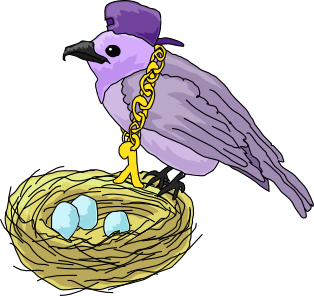
\includegraphics[scale=0.5]{images/nest.png}
    \end{center}
\end{frame}

\begin{frame}
    \frametitle{nesting your server methods}
    \begin{columns}[c]
    \column{.2\textwidth}
        
\includegraphics[scale=0.28]{images/all_the_way_down.png}
    \column{.8\textwidth}
        \begin{center}
        \fbox{\lstinputlisting{code/turtles/server.js}}
        \newline
        
        \huge
        nest your server function definitions
        
        \end{center}
    \end{columns}
\end{frame}

\begin{frame}
    \frametitle{nesting your client methods}
    \begin{columns}[c]
    \column{.2\textwidth}
        
\includegraphics[scale=0.28]{images/all_the_way_down.png}
    \column{.8\textwidth}
        \begin{center}
        \fbox{\lstinputlisting{code/turtles/client.js}}
        \newline
        
        \huge
        nest your client function definitions
        
        \end{center}
    \end{columns}
\end{frame}

\begin{frame}
    \frametitle{dnode in the wild}
    \begin{itemize}
    
    \item browserling.com - cross browser testing in your browser
    \pause
    
    \item github.com/Marak/JSONloops - multi-user audio sequencer
    \pause
    
    \item play.minespotter.com - realtime minesweeper clone
    \pause
    
    \item github.com/feisty/ToE - mmorpg
    \pause
    
    \item github.com/tanepiper/dnode-upload-example - realtime upload progress
    
    \end{itemize}
\end{frame}

\begin{frame}
    \frametitle{dnode in ruby}
    \begin{center}
        \huge
        github.com/substack/dnode-ruby
        \newline
        \normalsize
        \fbox{\lstinputlisting{code/client.rb}}
    \end{center}
\end{frame}

\begin{frame}
    \frametitle{dnode in perl}
    \begin{center}
        \huge
        github.com/substack/dnode-perl
        \newline
        \normalsize
        \fbox{\lstinputlisting{code/client.pl}}
    \end{center}
\end{frame}

\begin{frame}
    \frametitle{dnode in java?!}
    \begin{center}
        \huge
        github.com/aslakhellesoy/dnode-java
        \newline
        
\includegraphics[scale=0.6]{images/robot_stare.png}
    \end{center}
\end{frame}

\begin{frame}
    \frametitle{Git it!}
    \begin{center}
        \huge
        github.com/substack/dnode
        \newline
        
\includegraphics[scale=0.5]{images/robot.png}
    \end{center}
\end{frame}

\end{document}
